\documentclass{article}
\usepackage[utf8]{inputenc}

\title{5760 Project 1}
\author{Scott Carnahan}
\date{February 2019}

\usepackage{natbib}
\usepackage{graphicx}
\usepackage{amsmath}
\usepackage{float}
\usepackage[]{pdfpages}
\usepackage{siunitx}
\begin{document}

\maketitle
\tableofcontents

\section{Introduction}
For this project, I added a spherical reflective grating in place of the previous detector as well as a matched cylindrical detector along the grating's Rowland's Circle.  In the image below you'll see I made the detector exceedingly large in order ot be able to capture multiple diffraction orders.

\begin{figure}[H]
    \centering
    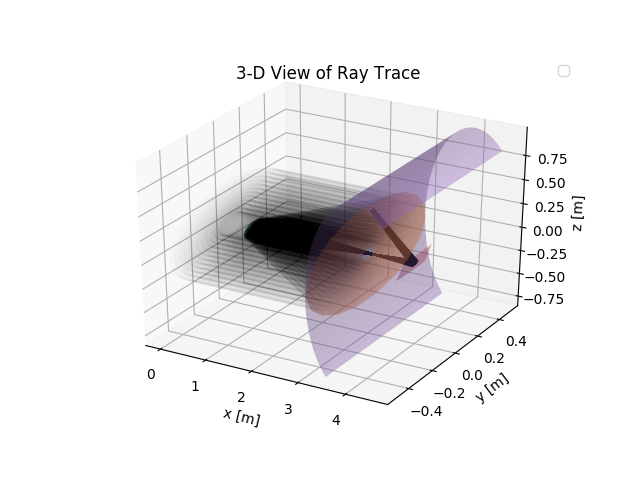
\includegraphics[width=10cm]{figures/lab_view.png}
    \caption{A 3d view of the ray trace with an impossibly large detector}
    \label{}



\end{figure}

\section{Diffraction Math}
First, we were asked to set $\beta$ to $0$. To do this, I focused on the center of the grating where I can treat it just as a flat grating with equal spacing. In that case, the grating equation reduces to:

\begin{equation}
    \sin{\alpha} = \frac{m \lambda}{d}
\end{equation}
where d for us is $1 / 3600$. I am assuming we are interested in the first order diffraction, as well. By inverting the sin, I got alpha. Now, with $\beta = 0$, a paraxial ray hitting the center of the grating would diffract along the normal of the spherical surface.  What I have to do is just rotate the sphere off-axis by $\alpha$.

The grating is placed with its vertex at $R\cos{\alpha}$ from the cassegrain focus. Then, the cylinder is placed along the Rowland's Circle with a diameter equal to the grating radius.

\subsection{Grating Math}
In order to keep my code vectorized, I followed the math by Spencer and Murty in \textit{General Ray Tracing Procedure}, 1961.  This treats the grating as the intersection of some virtual surfaces with the grating surface. If $\hat{p} = <u, v, w>$ is the normal of the virtual surfaces, then 
\begin{equation}
    u = \frac{1}{\sqrt{1 + \frac{K^2}{L^2 + M^2}}}
\end{equation}

where $\hat{r} = <K, L, M>$ is the surface normal of the sphere at a point. Then, the local line spacing $d$ is the parallel line space $d_p$, divided by $u$:

\begin{equation}
    \label{eq:local}
    d = d_p / u
\end{equation}

\subsection{Diffraction Direction}
The governing equation is
\begin{equation}
    \label{eq:fun}
    S^\prime = \mu S - \Lambda p + \Gamma r
\end{equation}
where $S$ is the direction vector in and $S^\prime$ is the direction out. $\Lambda$ is defined as $\frac{n\lambda}{N^\prime d}$ where the addition of $N^\prime$ has to do with refraction through non-similar mediums. $\Gamma$ is defined by a quadrati equation which the authors insist on iterating to a solution for a reason I don't understand. It incorporates the surface normal, beam direction, and grating direction.

\section{Spectrogram}
In order to contain my enthusiasm, I wrote the grating to only handle one wavelength and one order at a time. So, I looped over the wavelengths requested. Orders 0, 1, and 2 are shown on the graph. It's a bit large, but clear if zoomed in. The wavelengths travel angularly around the cylinder while the aberrations travel axially on the cylinder. The x-axis is in [radians] but this is equivalent to [meters] of circumference for this case. \bf{The image is included at the end of the file due to its size.}

\section{Limiting Resolving Power}
The limiting resolving power is given as
\begin{equation}
    \label{eq:resolve}
    R = \frac{\lambda}{\Delta \lambda}
\end{equation}
where $\lambda$ is the center wavelength and $\Delta \lambda$ is the minimum distinguishable wavelength different in the image.  For this, we can just assume that two wavelengths would need to be $100\%$ separated to achieve resolution, so we proceed:
\begin{equation}
    \label{eq:Amm}
    \frac{\si{\angstrom}}{mm} = \frac{10^7\cos{\beta}}{ml\frac{1}{d}}
\end{equation} which reduces to
\begin{equation}
    \label{eq:Ammred}
    \frac{\si{\angstrom}}{mm} = \frac{10^7 * 1}{1 * 1000 * 3600}
\end{equation} for our case and gives about 2.7. This is confirmed by measuring the mm between $100 \si{\angstrom}$ on the graph. Then, we multiply the resolution by the spread of a single wavelength line to estimate the resolving power.
\begin{equation}
    \label{eq:resolvingPower}
    R = \frac{\si{\angstrom}}{mm} \Delta \lambda \approx
\end{equation} The results are:
\begin{center}
    \input "../resolvingTable.txt"
\end{center}
Notably, the resolving power is probably better than this. This measure includes the width of the entire wavelegnth blob including the curve. This curve wouldn't actually run into other blobs because they too are curved. I would eyeball that the actual resolving power may be 5x better than this at the central wavelength, so maybe 30,000 - as long as diffraction didn't get in the way.

\eject \pdfpagewidth=22.5in \pdfpageheight=7.5in
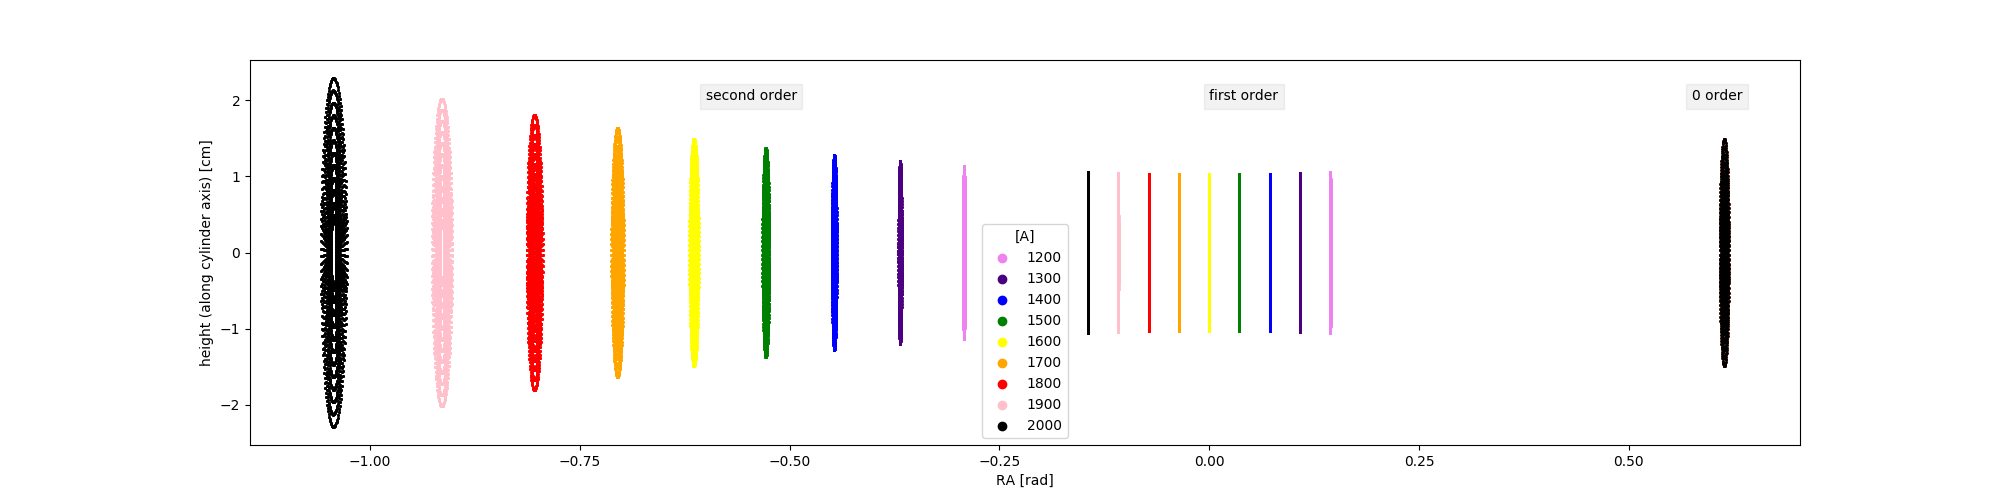
\includegraphics{figures/spectrum.png}


% \bibliograph\sin{\alpha} = \frac{m \lambda}{d}ystyle{plain}
% \bibliography{references}
\end{document}
